\documentclass[11.5pt, paper=a4]{article}

\usepackage[utf8]{inputenc}
\usepackage[english]{babel}
\usepackage[T1]{fontenc}

\usepackage{qcircuit}   



\usepackage{amsmath, amssymb, amscd, amsthm, amsfonts, mathtools}
\usepackage[left=2cm, right=2cm, top=1.5cm]{geometry}

\usepackage{graphicx}
\usepackage{hyperref}
\usepackage{physics}
\usepackage{tikz}
\usepackage{url}
\usepackage[square,numbers]{natbib} \usepackage{tabularx}

\usepackage{braket}
\usepackage{thmtools}
\usepackage{float}

\usepackage{tikz}
\usetikzlibrary{quantikz}

%%% Theorem Style
\theoremstyle{definition}
\newtheorem{theorem}{Theorem}[section]
\newtheorem{definition}[theorem]{Definition}
\newtheorem{lemma}[theorem]{Lemma}
\newtheorem{conjecture}[theorem]{Conjecture}
\newtheorem{corollary}[theorem]{Corollary}

\numberwithin{theorem}{section}

%% Autoref prefixes
\renewcommand{\sectionautorefname}{Section}
\renewcommand{\subsectionautorefname}{Section}
\renewcommand{\subsubsectionautorefname}{Section}
\renewcommand{\figureautorefname}{Figure}
\def\theoremautorefname{Theorem}
\def\lemmaautorefname{Lemma}
\def\definitionautorefname{Definition}
\def\conjectureautorefname{Conjecture}
\def\algorithmautorefname{Algorithm}

%% Writing algorithms

\usepackage{algorithm} % captioning 
\usepackage{algpseudocode}

% \def\NoNumber#1{{\def\alglinenumber##1{}\State #1}\addtocounter{ALG@line}{-1}}

\graphicspath{{./Lecture_13/images/}}


\title{Quantum Algorithms, Spring 2022: Lecture 13 Scribe}

\author{ Kushagra Garg, Pratishtha Abrol}

\date{February 24, 2022}

\begin{document}

\maketitle
\section{Recap}
In the previous lecture we looked at the circuit for modular exponentiation 
\begin{equation*}
    \ket{a}\ket{y} \xrightarrow{U_f} \ket{a}\ket{x^a y (mod N)}
\end{equation*}
We found out that it has complexity of $O(log^3N)$. Then we started with the Quantum Fourier Tranform. 


\begin{align*}
    \ket{j} \xrightarrow{QFT_N} & \frac{1}{\sqrt{N}}\sum_{k=0}^{N-1}e^{i2\pi jk/N} \ket{k} \\
    & = \frac{1}{\sqrt{N}} \left(\sum_{k_1=0}^{N-1}e^{i2\pi jk_1\times2^{n-1}/N} \ket{k_1}\right) 
    \left(\sum_{k_2=0}^{N-1}e^{i2\pi jk_2\times2^{n-2}/N} \ket{k_2}\right) \dots
    \left(\sum_{k_n=0}^{N-1}e^{i2\pi jk_n\times2^{0}/N} \ket{k_n}\right) \\
    &=  \frac{1}{\sqrt{N}} \bigotimes_{l=1}^n \sum_{k_l=0}^1 e^{i2\pi jk_l\times2^{-l}/N} \ket{k_l} \\
    &= \frac{1}{\sqrt{N}} \left(\ket{0} + e^{i2\pi j/2} \ket{1}\right)
     \left(\ket{0} + e^{i2\pi j/2^2} \ket{1}\right) \dots
      \left(\ket{0} + e^{i2\pi j/2^n} \ket{1}\right) \\
      &= \frac{1}{\sqrt{N}} \left(\ket{0} + e^{i2\pi 0.j_n} \ket{1}\right)
     \left(\ket{0} + e^{i2\pi 0.j_{n-1}j_n} \ket{1}\right) \dots
      \left(\ket{0} + e^{i2\pi 0.j_1 \dots j_n \ket{1}}\right) 
\end{align*}
We will now look at the circuit for the QFT. 
\section{Quantum Fourier Transform Circuit}
The elementary gates that we use are the Hadamards and the controlled-$R_x$ gates, where 
$R_X = 
\begin{pmatrix}
1 & 0 \\
0 & e^{2\pi i /2^x}
\end{pmatrix}
$

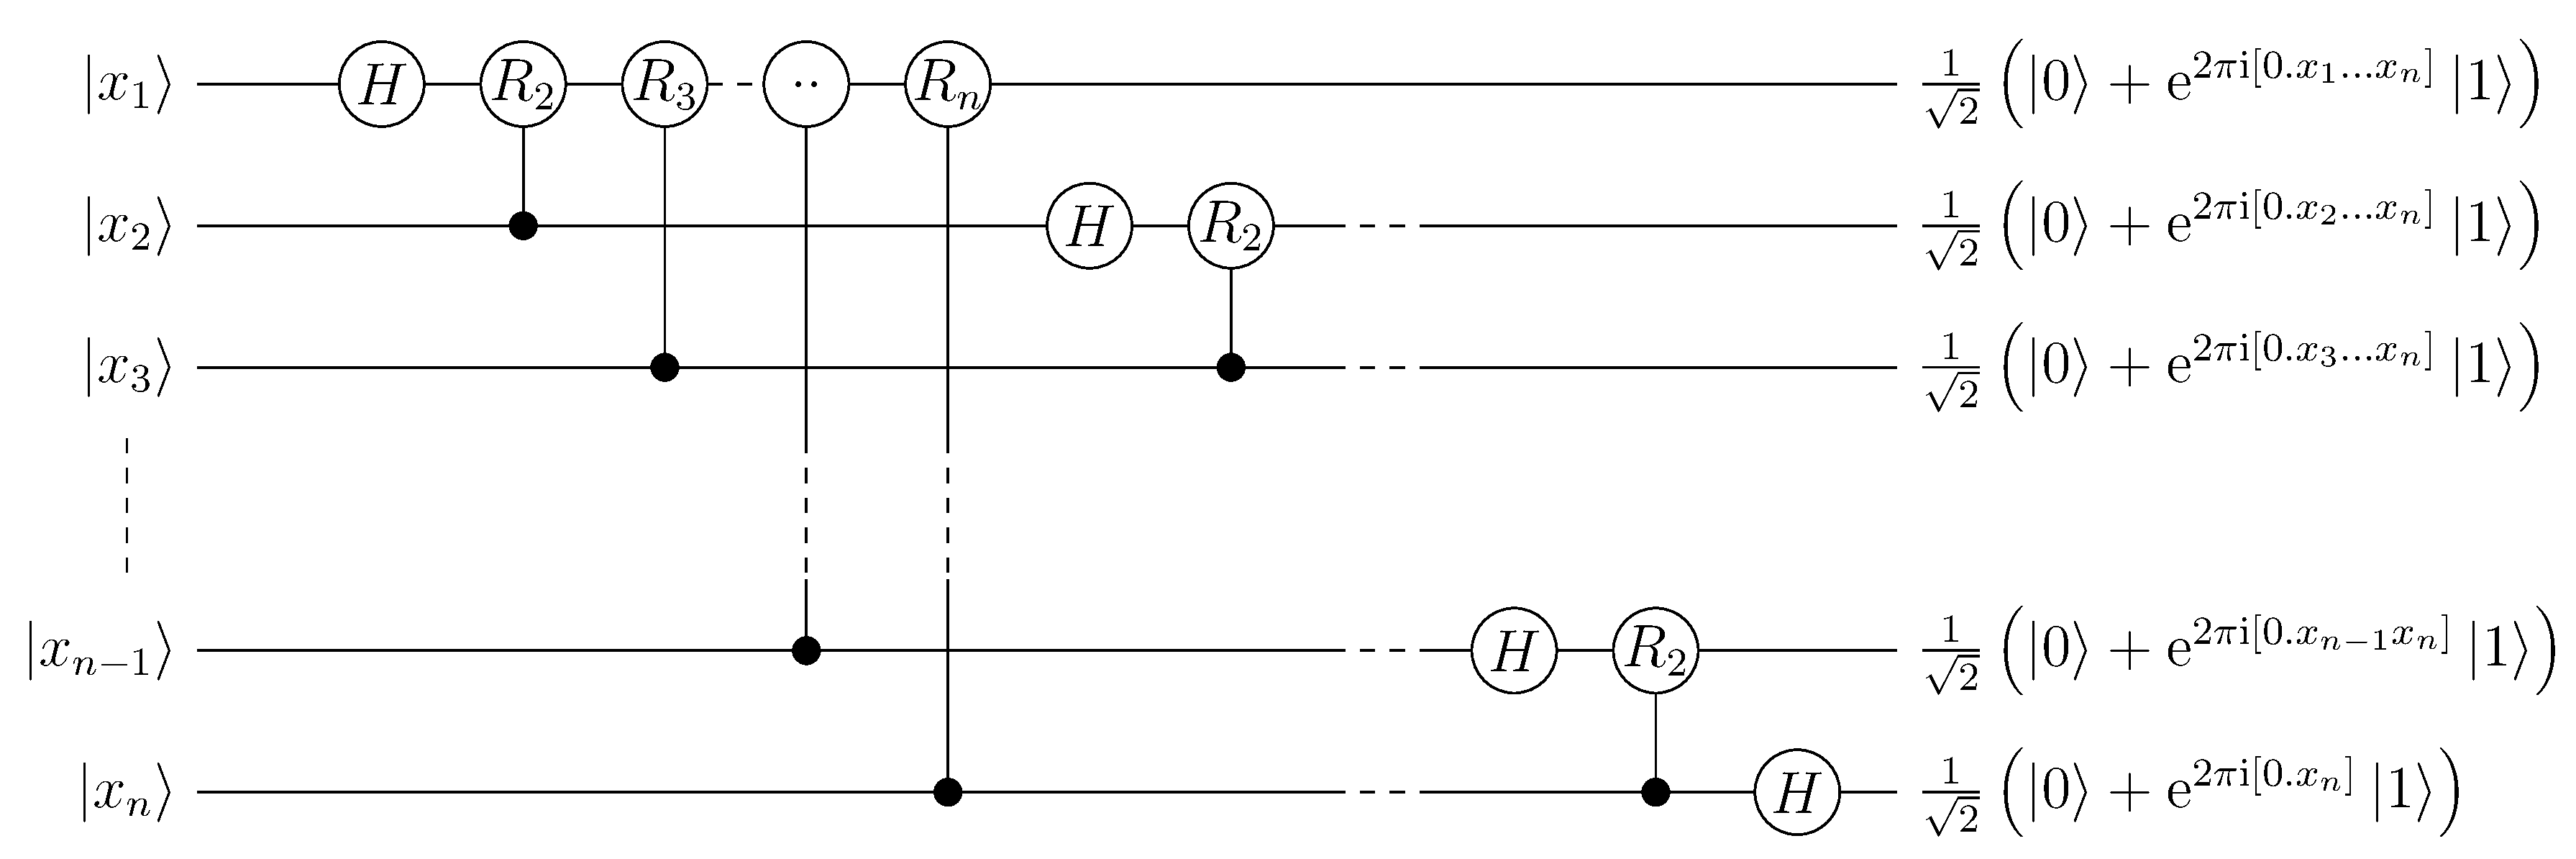
\includegraphics[width=15cm, height=6cm]{images/qft_circuit.png}

\subsection{Complexity of QFT}

\begin{itemize}
    \item Hadamard Gates: $n$
    \item SWAP Gates: $n/2$
    
\end{itemize}

\text{Total Complexity} $= O(\log^2N) $
\section{Quantum Phase Estimation}
Suppose $U$ is a unitary with eigenvector $\ket{v}$ and an eigenvalue $e^{2\pi\theta}$ where $0\leq \theta \le 1$. Suppose the cost of implementing $U$ is $T_U$. Then given $\ket{v}$ (this assumption will be droped later) there exists a quantum algorithm that outputs $\Tilde{\theta}$ such that $|\Tilde{\theta} - \theta| \leq \epsilon$, with success probability  $\geq 1-\delta$ in time $T = O\big(\frac{T_U}{\delta\epsilon}\big)$
\newline

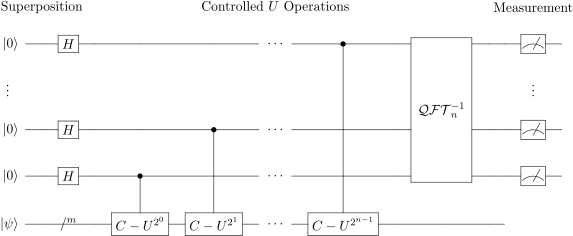
\includegraphics[width=16cm, height=6cm]{images/PhaseCircuit-crop.png}
\vspace{0.5cm}
\\ Let us assume that there are n qubits in register 1. The choice of n will depend on the accuracy with which we estimate $\theta$ as well as on the success probability. 

\begin{itemize}
    \item We start with the state
    
    $$
    \ket{\psi_0} = \ket{0}^{\otimes n}\ket{\psi}
    $$
    
    where $\psi$ is the eigenvector of our unitary. 
    
    \item On applying a n-bit Hadamard gate operation $H^{\otimes n}$ on the counting register we get
    
    $$
        \ket{\psi_1} = \frac{1}{2^{n/2}} (\ket{0}+\ket{1})^{\otimes n}\ket{\psi}
    $$
    
    \item Then we apply the  n controled rotations as shown in circuit. We use the relationship 
    $$
    \ket{0} \otimes \ket{\psi} + \ket{1} \otimes e^{2\pi i \theta}\ket{\psi} = (\ket{0} + e^{2\pi i \theta}\ket{1})\otimes \ket{\psi}
    $$
    We get the state
    
    $$
    \begin{aligned}
        \ket{\psi_2} &= \frac{1}{2^{n/2}} (\ket{0} + e^{2\pi i \theta 2^{n-1}}\ket{1}) \otimes \dots \otimes (\ket{0} + e^{2\pi i \theta 2}\ket{1})\otimes (\ket{0} + e^{2\pi i \theta})\ket{1} \\
        &= \frac{1}{2^{n/2}} \sum_{k = 0}^{2^n -1 }e^{2\pi i \theta k }\ket{k} \otimes \ket{\psi}
    \end{aligned}
    $$
    
    Observe That it is Quantum Fourier Transform of the theta vector.
    
    \item We then apply the Inverse Fourier transformation to get the $\theta$ state. 
    
    $$
    \ket{\psi_3} = = \frac{1}{2^{n/2}} \sum_{k = 0}^{2^n -1 }e^{2\pi i \theta k }\ket{k} \otimes \ket{\psi} \xrightarrow{QFT^{-1}} \sum_{k = 0}^{2^n -1 } \sum_{k = 0}^{2^n -1 } e^{\frac{2\pi i k}{2^n}(x - 2^n\theta) }\ket{x} \otimes \ket{\psi}
    $$
    
    If $\theta$ can exactly be expressed in $n$-qubits i.e.   $x = 2^n\theta$ then measuring in the computational basis gives the phase in the auxiliary register with high probability:
    
    \par For the case when $2^n \theta$ is not an integer, we will show that above expression still peaks near $x = 2^n\theta$ with probability better than $4/\pi^2$
    
    \par let $\theta = \frac{x}{2^n} + \delta$ where $0 \le |\delta| \leq \frac{1}{s^{t+1}}$. The final state that we get can be written as 
    
    $$
    \ket{\psi_3} = \frac{1}{2^n} \sum_{k = 0}^{2^n -1}\sum_{x = 0}^{2^n -1}e^{2\pi ik (\theta - x/2^n) }\ket{x}
    $$
    
    On measuring this register:
    
    $$
        |r_x|^2 = |\frac{1}{2^n}  \sum_{k = 0}^{2^n -1}e^{2\pi ik\delta }|^2
    $$
    Let $T = 2^n$
    
    $$
    \begin{aligned}
        |r_x|^2 = \frac{1}{T^2} \frac{|1- e^{i2\pi T \delta}|^2}{|1- e^{i2\pi \delta}|^2}\\
        &= \frac{1}{T^2} \frac{\sin^2(\pi T \delta)}{\sin^2(\pi \delta)}
    \end{aligned}
    $$
    
    As $0 \leq \delta \leq \frac{1}{2^{n+1}}$ then $0\leq \pi \delta T \leq \pi/2$
    
    using 
    $$
        \sin^2x \leq x, x \in \mathcal{R} \\
        \sin x \geq 2x/\pi, x \in (0, \pi/2]
    $$
    we get
    $$
        |r_x|^2 \geq \frac{(2 \pi T \delta / \pi)^2}{\pi^2 \delta^2 T^2} = \frac{4}{\pi^2}
    $$
    
    \textbf{Next Lecture:} We want to use QPE as an intermediate step in other algorithm so constant success probability is not enough. We will find the value for 'n' to get 'd' bit approximation of $\theta$ s.t. $|\Tilde{\theta} - \theta| \leq \epsilon$, with success probability  $\geq 1-\delta$.
\end{itemize}


\bibliographystyle{plainnat}

\end{document}

